\documentclass{beamer}
\mode<presentation>
\usetheme{CambridgeUS}
\usepackage[russian]{babel}
\usepackage[utf8]{inputenc}
\usepackage[T2A]{fontenc}
\usepackage{sansmathaccent}

\usepackage{verbatim}
\usepackage{alltt}

\pdfmapfile{+sansmathaccent.map}
\title[Текстовые файлы]{Текстовые и нетипизированные файлы}
\author{Наумов Д.А., доц. каф. КТ}
\date[05.05.2020] {Программирование и алгоритмические языки, 2020}

\setbeamertemplate{caption}[numbered] % Нумерация рисунков в презентации

\begin{document}

\begin{frame}
  \titlepage
\end{frame}
  
\begin{frame}
  \frametitle{Содержание лекции}
  \tableofcontents  
\end{frame}
  
\section{Файлы и файловый тип данных}

\begin{frame}
\begin{block}{Файл}
именованная сущность, для которой определены операции ввода и вывода данных.
\end{block}
Для работы с файлами в Pascal предусмотрены \textbf{файловые типы данных}:
\begin{enumerate}
\item типизированные: информация считывается и записывается в переменные конкретного типа (целые, вещественные, массивы и т. д.);
\item нетипизированные: информация считывается и записывается блоками определённого размера.
\item текстовые: информация обрабатывается посимвольно, но возможно чтение и запись данных в переменные строкового, целого и вещественного типа.
\end{enumerate}
\end{frame} 

\section{Нетипизированные файлы}

\begin{frame}
%  \frametitle{Содержание лекции}
  \tableofcontents[currentsection]
\end{frame}

\begin{frame}[fragile]{Описание переменной файлового типа нетипизированного файла}
Для описания файловой переменной нетипизированного файла используется  ключевое слово \textbf{file} без обозначения типа элементов.
\begin{alltt}
//описание переменных файлового типа
1 var                  
2   F1: file; //это - нетипизированный файл
\end{alltt}
Файл без типа можно представить как последовательность элементов произвольного типа, но заданного размера.
\end{frame}

\begin{frame}[fragile]{Подпрограммы работы с нетипизированными файлами}
Для нетипизированных файлов доступны все те же процедуры и функции, что и для типизированных файлов, за исключением:
\begin{itemize}
\item процедуры Reset и Rewrite имеют расширенный синтаксис:
\item вместо процедур чтения и записи (Read, Write) необходимо использовать процедуры BlockWrite и BlockRead:
\end{itemize}
Синтаксис процедур открытия файлов:
\begin{alltt}
Reset(var f: File; BuferSize: word);
Rewrite(var f: File; BuferSize: word) ;
\end{alltt}
\begin{itemize}
\item Второй параметр BuferSize операторов Reset и Rewrite может быть опущен, что означает задание размера записи в 128 байт. 
\item Наибольшая скорость обмена данными обеспечивается при длине записи, кратной размеру сектора на диске.
\end{itemize}
\end{frame}

\begin{frame}[fragile]{Подпрограммы работы с нетипизированными файлами}
\begin{block}{Процедура BlockWrite}
запись данных в нетипизированный файл.
\end{block}
Синтаксис: BlockWrite(var f: file; var X; Count: word; var WriteCount: word);
\begin{block}{Процедура BlockRead(f)}
чтение данных из нетипизированного файла.
\end{block}
Синтаксис: BlockRead(var f: file; var X; Count: word; var ReadCount: word);
\begin{itemize}
\item f - переменная файлового типа;
\item x - переменная произвольного типа;
\item Count - количество блоков памяти размером BuferSize;
\item ReadCount(WriteCount) - количество считанных (записанных) блоков.
\end{itemize}
\end{frame}

\begin{frame}[fragile]{Пример копирования файла при помощи нетипизированных файлов}
\begin{alltt}
var SourceFile, DestFile: file; //файловые переменные
  SourceFileName, DestFileName: string; //имена файлов
  ReadCount, WriteCount: word; 
  Buffer: array[1..BUFFER_SIZE] of byte; // буфер
begin
  ReadLn(SourceFileName, DestFileName);  
  Assign(SourceFile, SourceFileName);
  \{$I-\}Reset(SourceFile, 1);\{$I+\}
  if IOResult <> 0 then begin
    WriteLn('Error while opening file ', SourceFileName);
    Halt(1);
  end;
  Assign(DestFile, DestFileName);
  Rewrite(DestFile, 1);
\end{alltt}
\end{frame}

\begin{frame}[fragile]{Пример копирования файла}
\begin{alltt}
  Error := erOK;
  repeat
    BlockRead(SourceFile, Buffer, BUFFER_SIZE, ReadCount);
    if ReadCount = 0 then begin
      Error := erReadError;
      break;
    end;
    BlockWrite(DestFile, Buffer, ReadCount, WriteCount);
    if ReadCount <> WriteCount then begin
      Error := erWriteError;
      break;
    end;
  until EOF(SourceFile);
  Close(SourceFile); 
  Close(DestFile);
\end{alltt}
\end{frame}

\section{Операции с текстовыми файлами}
\begin{frame}
%  \frametitle{Содержание лекции}
  \tableofcontents[currentsection]
\end{frame}

\begin{frame}[fragile]{Описание переменной тестового файла}
Для описания файловой переменной текстового файла используется специальный тип данных - \textbf{text}.
\begin{alltt}
//описание переменных файлового типа
1 var                  
2   F1: text; //это - текстовый файл
3   F2: file of char; //это - типизированный файл,
                      //он не является текстовым
\end{alltt}
Несмотря на то, что данные из файлов F1 и F2 могут быть считаны посимвольно, для текстовых файлов доступны некоторые специфические функции и процедуры, и по-разному обрабатываются символы перехода на новую строку (символ с кодом 10 или два символа с кодом 10, 13). 
\end{frame}

\begin{frame}[fragile]{Операции с текстовыми файлами}
С текстовыми файлами работают процедуры и функции, описанные в предыдущей лекции:
\begin{itemize}
\item Assign(F, s) - связь файла и файловой переменной;
\item Reset(F) - открытие файла для чтения;
\item Rewrite(F) - открытие файла для перезаписи;
\item Close(F) - закрытие файла;
\item Rename(F) - переименование файла;
\item Erase(F) - удаление файла;
\item EOF(F) - проверка на достижения конца файла;
\end{itemize}
Подпрограммы, которые недоступны для работы с текстовыми файлами:
\begin{itemize}
\item Функция Filesize(f)
\item Функция Filepos(f)
\item Процедура Seek(f, k)
\item Процедура Truncate(f)
\end{itemize}
\end{frame} 

\begin{frame}[fragile]{Открытие файла}
Для текстового файла имеется еще одна процедура открытия:
\begin{block}{Процедура Append}
открывает текстовый файл для дозаписи.
\end{block}
Синтаксис: Append(f)
\begin{itemize}
\item f - переменная текстового файла;
\item файл должен существовать;
\item текущей позицией для записи становится конец файла.
\end{itemize}
\begin{alltt}
 1 var                  
 2   F1: text;
 3 begin
 4   Assign(F1, 'myfile.txt');
 5   Append(F1);
\end{alltt}
\end{frame} 

\begin{frame}[fragile]{Чтение из файла}
\begin{block}{Процедура Read}
выполняет чтение информации из текстового или типизированного файла.
\end{block}
Синтаксис: Read(f, x1, x2, x3, $...$, xn);
\begin{itemize}
\item f - переменная файлового типа;
\item x1, x2, x3, $...$, xn - переменные.
\end{itemize}
Для текстового файла можно считывать значения:
\begin{itemize}
\item символьного, 
\item целого, 
\item вещественного, 
\item строкового типов 
\item и отрезков символьного и целого типов.
\end{itemize} 
\end{frame} 

\begin{frame}[fragile]{Запись в файл}
\begin{block}{Процедура Write}
выполняет запись информации в текстовый или типизированный файл.
\end{block}
Синтаксис: Write(f, x1, x2, x3, $...$, xn);
\begin{itemize}
\item f - переменная файлового типа;
\item x1, x2, x3, $...$, xn - переменные.
\end{itemize}
Для текстового файла можно записывать значения символьного, целого, вещественного, строкового типов (и отрезков символьного и целого типов).
\end{frame} 

\begin{frame}[fragile]
\begin{block}{Процедура Readln}
выполняет чтение из текстового файла до символа конца строки. Символ конца строки считывается из файла, но не добавляется его в считываемые данные.
\end{block}
Синтаксис: Readln(f, x1, x2, x3, $...$, xn);
\begin{itemize}
\item f - переменная файлового типа;
\item x1, x2, x3, $...$, xn - переменные.
\end{itemize}
\begin{block}{Процедура Writeln}
выполняет запись в текстовый файл и добавляет символ конца строки.
\end{block}
Синтаксис: Writeln(f, x1, x2, x3, $...$, xn);
\begin{itemize}
\item f - переменная файлового типа;
\item x1, x2, x3, $...$, xn - переменные.
\end{itemize}
\end{frame}

\section{Примеры работы с текстовыми файлами}
\begin{frame}
%  \frametitle{Содержание лекции}
  \tableofcontents[currentsection]
\end{frame}

\begin{frame}[fragile]
Пусть в текстовом файле содержится информация о двумерном массиве. Первые два числа содержат данные о размерности (4х3), остальные данные - это значения элементов двумерного массива:
\begin{alltt}
4 3
-1 6 3 
-4 8 12 
3 15 9
4 -2 6
\end{alltt}
Удобным механизмом, который можно использовать в задачах, где размерность данных заранее неизвестна, являются открытые массивы, (динамические массивы, для которых не указан тип индекса). 
\begin{alltt}
type
  TVector = array of real; //одномерный массив TVector
  TMatrix = array of TVector; //массив из векторов
var
  V: TVector;
  M: TMatrix;
\end{alltt}
\end{frame}

\begin{frame}[fragile]
Так как массивы являются динамическими, то их размер должен быть задан в процессе выполнения при помощи процедуры SetLength() следующего синтаксиса:
\begin{alltt}
   SetLength(Массив, Размер)
\end{alltt}
\begin{itemize}
\item Массив - переменная типа динамического массива;
\item Размер - целое число, количество элементов массива.
\end{itemize}
После того, как размер массива задан, можно получить доступ к его элементам. Доступ осуществляется при помощи операции индексации, элементы нумеруются целыми значениями, начиная с нуля.
\begin{alltt}
  SetLength(V, 10); //задаем размер, равный 10
  for i := 0 to High(V) do
    V[i] := random;
\end{alltt}
Индекс последнего элемента можно узнать при помощи функции High().
\end{frame}

\begin{frame}[fragile]
Рассмотрим чтение данных из текстового файла в двумерный массив.
\begin{alltt}
var
  F: Text; //текстовый файл входных данных
  var M:TMatrix; //массив
  i, j: TIndex; //индексы
  Rows, Cols: TIndex; //количество строк и столбцов
begin
  //связываем файл и файловую переменную
  Assign(F, FileName);
  \{$I-\}
  Reset(F); //открываем файл для чтения
  \{$I+\}
  if IOResult <> 0 then //если возникла ошибка
  begin                 
    //то файл не существует, завершаем работу
    WriteLn('Error: file not found');
    halt;
  end;
\end{alltt}
\end{frame}

\begin{frame}[fragile]
\begin{alltt}
  //первые два элемента - это количество строк и столбов
  \{$I-\}
  Readln(F, Rows, Cols);
  \{$I+\}
  //если не удалось считать значения
  if IOResult <> 0 then
  begin
    WriteLn('Error: Data error');
    halt;
  end;
  //если размеры меньше 1 - ошибка
  if (Rows < 1) or (Cols < 1) then
  begin
    WriteLn('Error: Bad array size');
    halt;
  end;
\end{alltt}
\end{frame}

\begin{frame}[fragile]
\begin{alltt}
  //задаем размер массива
  SetLength(M, Rows);
  //задаем размер всех строк
  for i := 0 to Rows-1 do
    SetLength(M[i], Cols); 
  //читаем данные из файла
  for i := 0 to Rows-1 do
  begin
    for j := 0 to Cols-1 do
    \{$I-\}Read(F, M[i][j]);\{$I+\}
    //если не удалось считать значение
    if IOResult <> 0 then
    begin
      WriteLn('Error: Data error');
      halt;
    end;
  end;  
  Close(F); //закрываем файл 
\end{alltt}
\end{frame}

\section{Работа с аргументами программы}
\begin{frame}
%  \frametitle{Содержание лекции}
  \tableofcontents[currentsection]
\end{frame}

\begin{frame}[fragile]{Работа с аргументами программы}
\begin{enumerate}
\item При запуске (через командную строку или из другой программы) программе могут передаваться аргументы, которые затем программа может обработать и использовать.
\item В аргументах могут быть заданы настройки, имена файлов входных и выходных данных и другие опции.
\item Большинство утилит операционной системы (как семейства Windows, так и семества Linux) запускаются из командной строки и настраиваются при помощи задаваемых аргументов. 
\end{enumerate}
\begin{center}
\begin{figure}
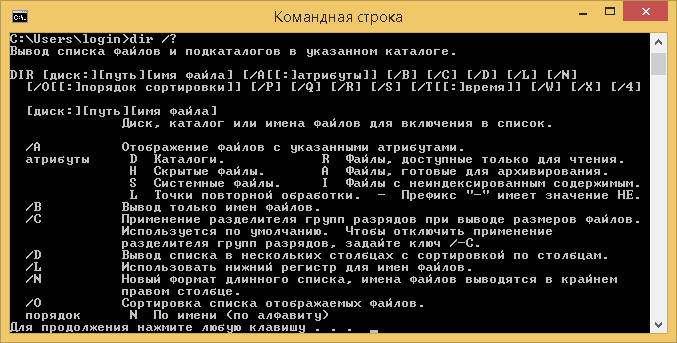
\includegraphics[scale=0.3]{images/lec13-pic01.png}
\caption{Пример списка аргументов утилиты DIR}
\end{figure}
\end{center}
\end{frame}

\begin{frame}[fragile]{Работа с аргументами программы}
Пусть программа (scalar\_prod.exe) должна считать из файлов два вектора, найти их скалярное произведение и вывести результат в текстовый файл.

Тогда, необходимы три аргумента:
\begin{itemize}
\item имя первого входного файла;
\item имя второго входного файла;
\item имя файла результатов.
\end{itemize}

Запуск может осуществляться следующим образом:
\begin{alltt}
   scalar\_prod.exe file1.txt file2.txt result.txt
\end{alltt}
\end{frame}

\begin{frame}[fragile]{Работа с аргументами программы}
Для доступа к аргументам программы в языке Pascal используются следующие функции:
\begin{itemize}
\item function ParamCount: integer - получить количество аргументов программы;
\item function ParamStr(ParamNumber: integer): string - получить значение аргумента с номером ParamNumber.
\end{itemize}
Пример вывода всех аргументов командной строки:
\begin{alltt}
for i := 1 to ParamCount do
  WriteLn('Param number ', i, ' is ', ParamStr(i));
\end{alltt}
При обработке аргументов командной строке желательно предусмотреть возможность запуска программы с аргументом $'\backslash h'$ или $'\backslash ?'$ для вывода подсказки в случае, если пользователь не знает, как именно необходимо запускать программу, а также вывод справки при запуске программы без аргументов.
\end{frame}

\begin{frame}[fragile]
Проверка аргументов командной строки для программы scalar\_prod: \begin{alltt}
  if ParamCount = 1 then
    if (ParamStr(1)= '\textbackslash\hspace{0pt}h') or (ParamStr(1)= '\textbackslash?') then begin
      Writeln('Использование программы:');
      Writeln('   scalar\_prod file1 file2 result');
      Writeln('   file1 - имя входного файла для вектора V1');
      Writeln('   file2 - имя входного файла для вектора V2');      
      Writeln('   result - имя файла результатов');   
    end
    else Writeln('Запустите программу с ключом '\textbackslash?'')
  else
    if ParamCount <> 3 then
      Writeln('Запустите программу с ключом '\textbackslash?'')
    else begin
      FileName1 := ParamStr(1);
      FileName2 := ParamStr(2);
      ResultFileName := ParamStr(3);      
    end;
\end{alltt}
\end{frame}

\begin{frame}[fragile]
Для запуска программы из среды Lazarus необходимо настроить параметры командной строки при помощи окна "Параметры запуска", вызываемого при помощи меню "Запуск - Параметры запуска"
\begin{center}
\begin{figure}
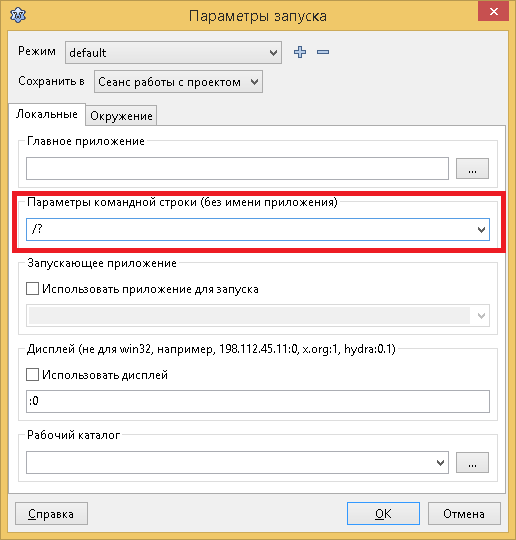
\includegraphics[scale=0.4]{images/lec13-pic06.png}
\caption{Окно настройки параметров командной строки в Lazarus}
\end{figure}
\end{center}
\end{frame}

\end{document}
